%%%% Paramétrage du TD %%%%
\def\xxactivite{\ifcolle Colle \else Application 03 \fi \ifprof -- Corrigé \else \fi }
\def\xxauteur{\textsl{Xavier Pessoles}}


\def\xxnumchapitre{Révisions 4 \vspace{.2cm}}
\def\xxchapitre{\hspace{.12cm} Modélisation des systèmes du premier et du deuxième ordre}

\def\xxcompetences{%
\vspace{-.5cm}
\footnotesize{
\textsl{%
\textbf{Savoirs et compétences :}\\
\vspace{-.2cm}
\begin{itemize}[label=\ding{112},font=\color{ocre}] 
\item ...
\end{itemize}}}}

\def\xxfigures{
%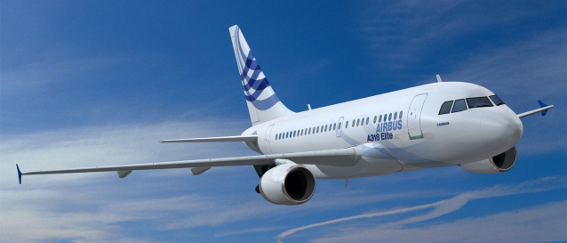
\includegraphics[width=.8\linewidth]{image1.png}%images/prot_01}
}%figues de la page de garde

\def\xxonglet{\textsf{Cy 01 -- Rév 4}}

\def\xxtitreexo{Robot de maraîchage Oz 440}
\def\xxsourceexo{CCP -- MP -- Florestan Mathurin}

\iflivret
\pagestyle{empty}


%%%%%%%% PAGE DE GARDE COURS
\ifcours
% ==== BANDEAU DES TITRES ==== 
\begin{tikzpicture}[remember picture,overlay]
\node at (current page.north west)
{\begin{tikzpicture}[remember picture,overlay]
\node[anchor=north west,inner sep=0pt] at (0,0) {\includegraphics[width=\paperwidth]{\thechapterimage}};
\draw[anchor=west] (-2cm,-8cm) node [line width=2pt,rounded corners=15pt,draw=ocre,fill=white,fill opacity=0.6,inner sep=40pt]{\strut\makebox[22cm]{}};
\draw[anchor=west] (1cm,-8cm) node {\huge\sffamily\bfseries\color{black} %
\begin{minipage}{1cm}
\rotatebox{90}{\LARGE\sffamily\textsc{\color{ocre}\textbf{\xxnumpartie}}}
\end{minipage} \hfill
\begin{minipage}[c]{14cm}
\begin{titrepartie}
\begin{flushright}
\renewcommand{\baselinestretch}{1.1} 
\Large\sffamily\textsc{\textbf{\xxpartie}}
\renewcommand{\baselinestretch}{1} 
\end{flushright}
\end{titrepartie}
\end{minipage} \hfill
\begin{minipage}[c]{3.5cm}
{\large\sffamily\textsc{\textbf{\color{ocre} \discipline}}}
\end{minipage} 
 };
\end{tikzpicture}};
\end{tikzpicture}
% ==== FIN BANDEAU DES TITRES ==== 


% ==== ONGLET 
\begin{tikzpicture}[overlay]
\node[shape=rectangle, 
      rounded corners = .25 cm,
	  draw= ocre,
	  line width=2pt, 
	  fill = ocre!10,
	  minimum width  = 2.5cm,
	  minimum height = 3cm,] at (18.3cm,0) {};
\node at (17.7cm,0) {\rotatebox{90}{\textbf{\Large\color{ocre}{\classe}}}};
%{};
\end{tikzpicture}
% ==== FIN ONGLET 


\vspace{3.5cm}

\begin{tikzpicture}[remember picture,overlay]
\draw[anchor=west] (-2cm,-6cm) node {\huge\sffamily\bfseries\color{black} %
\begin{minipage}{2cm}
\begin{center}
\LARGE\sffamily\textsc{\color{ocre}\textbf{\xxactivite}}
\end{center}
\end{minipage} \hfill
\begin{minipage}[c]{15cm}
\begin{titrechapitre}
\renewcommand{\baselinestretch}{1.1} 
\Large\sffamily\textsc{\textbf{\xxnumchapitre}}

\Large\sffamily\textsc{\textbf{\xxchapitre}}
\vspace{.5cm}

\renewcommand{\baselinestretch}{1} 
\normalsize\normalfont
\xxcompetences
\end{titrechapitre}
\end{minipage}  };
\end{tikzpicture}
\vfill

\begin{flushright}
\begin{minipage}[c]{.3\linewidth}
\begin{center}
\xxfigures
\end{center}
\end{minipage}\hfill
\begin{minipage}[c]{.6\linewidth}
\startcontents
%\printcontents{}{1}{}
\printcontents{}{1}{}
\end{minipage}
\end{flushright}

\begin{tikzpicture}[remember picture,overlay]
\draw[anchor=west] (4.5cm,-.7cm) node {
\begin{minipage}[c]{.2\linewidth}
\begin{flushright}

\includegraphics[width=2cm]{logoCC}
\end{flushright}
\end{minipage}
\begin{minipage}[c]{.2\linewidth}
\textsl{\xxauteur} \\
\textsl{\classe}
\end{minipage}
 };
\end{tikzpicture}

\newpage
\pagestyle{fancy}

%\newpage
%\pagestyle{fancy}

\else
\fi
%% FIN PAGE DE GARDE DES COURS

%%%%%%%% PAGE DE GARDE TD
\iftd

% BANDEAU EXO
\iflivret % SI LIVRET
\begin{tikzpicture}[remember picture,overlay]
\draw[anchor=west] (-2cm,-3.3cm) node {\huge\sffamily\bfseries\color{black} %
\begin{minipage}{5cm}
\begin{center}
\LARGE\sffamily\color{ocre}\textbf{\textsc{\xxactivite}}

\begin{center}
\xxfigures
\end{center}

\end{center}
\end{minipage} \hfill
\begin{minipage}[c]{12cm}
\begin{titrechapitre}
\renewcommand{\baselinestretch}{1.1} 
\large\sffamily\textbf{\textsc{\xxtitreexo}}

\small\sffamily{\textbf{\textit{\color{black!70}\xxsourceexo}}}
\vspace{.5cm}

\renewcommand{\baselinestretch}{1} 
\normalsize\normalfont
\xxcompetences
\end{titrechapitre}
\end{minipage}};
\end{tikzpicture}
\else % ELSE NOT LIVRET
\begin{tikzpicture}[remember picture,overlay]
\draw[anchor=west] (-2cm,-4.5cm) node {\huge\sffamily\bfseries\color{black} %
\begin{minipage}{5cm}
\begin{center}
\LARGE\sffamily\color{ocre}\textbf{\textsc{\xxactivite}}

\begin{center}
\xxfigures
\end{center}

\end{center}
\end{minipage} \hfill
\begin{minipage}[c]{12cm}
\begin{titrechapitre}
\renewcommand{\baselinestretch}{1.1} 
\large\sffamily\textbf{\textsc{\xxtitreexo}}

\small\sffamily{\textbf{\textit{\color{black!70}\xxsourceexo}}}
\vspace{.5cm}

\renewcommand{\baselinestretch}{1} 
\normalsize\normalfont
\xxcompetences
\end{titrechapitre}
\end{minipage}};
\end{tikzpicture}

\fi

\else   % FIN IF TD
\fi


%%%%%%%% PAGE DE GARDE FICHE
\iffiche
\begin{tikzpicture}[remember picture,overlay]
\node at (current page.north west)
{\begin{tikzpicture}[remember picture,overlay]
\draw[anchor=west] (-2cm,-2.25cm) node [line width=2pt,rounded corners=15pt,draw=ocre,fill=white,fill opacity=0.6,inner sep=40pt]{\strut\makebox[22cm]{}};
\draw[anchor=west] (1cm,-2.25cm) node {\huge\sffamily\bfseries\color{black} %
\begin{minipage}{1cm}
\rotatebox{90}{\LARGE\sffamily\textsc{\color{ocre}\textbf{\xxnumpartie}}}
\end{minipage} \hfill
\begin{minipage}[c]{14cm}
\begin{titrepartie}
\begin{flushright}
\renewcommand{\baselinestretch}{1.1} 
\large\sffamily\textsc{\textbf{\xxpartie} \\} 

\vspace{.2cm}

\normalsize\sffamily\textsc{\textbf{\xxnumchapitre -- \xxchapitre}}
\renewcommand{\baselinestretch}{1} 
\end{flushright}
\end{titrepartie}
\end{minipage} \hfill
\begin{minipage}[c]{3.5cm}
{\large\sffamily\textsc{\textbf{\color{ocre} \discipline}}}
\end{minipage} 
 };
\end{tikzpicture}};
\end{tikzpicture}

\iflivret % SI LIVRET
\begin{tikzpicture}[overlay]
\node[shape=rectangle, 
      rounded corners = .25 cm,
	  draw= ocre,
	  line width=2pt, 
	  fill = ocre!10,
	  minimum width  = 2.5cm,
	  minimum height = 2.5cm,] at (18.5cm,.5cm) {};
\node at (17.9cm,.5cm) {\rotatebox{90}{\textsf{\textbf{\large\color{ocre}{\classe}}}}};
%{};
\end{tikzpicture}
\else  % SI PAS LIVRET
\iftd %% SI TD et PAS LIVRET
\begin{tikzpicture}[overlay]
\node[shape=rectangle, 
      rounded corners = .25 cm,
	  draw= ocre,
	  line width=2pt, 
	  fill = ocre!10,
	  minimum width  = 2.5cm,
	  minimum height = 2.5cm,] at (18.6cm,0.9cm) {};
\node at (18cm,0.9cm) {\rotatebox{90}{\textsf{\textbf{\large\color{ocre}{\classe}}}}};
%{};
\end{tikzpicture}

\else % FIN DU SI TD PAS LIVRET 
\begin{tikzpicture}[overlay]
\node[shape=rectangle, 
      rounded corners = .25 cm,
	  draw= ocre,
	  line width=2pt, 
	  fill = ocre!10,
	  minimum width  = 2.5cm,
%	  minimum height = 2.5cm,] at (18.5cm,1.1cm) {};
	  minimum height = 2.5cm,] at (18.6cm,0.5cm) {};
\node at (18cm,0.5cm) {\rotatebox{90}{\textsf{\textbf{\large\color{ocre}{\classe}}}}};
%{};
\end{tikzpicture}
\fi
\fi
\else
\fi



\else
\pagestyle{empty}


%%%%%%%% PAGE DE GARDE COURS
\ifcours
% ==== BANDEAU DES TITRES ==== 
\begin{tikzpicture}[remember picture,overlay]
\node at (current page.north west)
{\begin{tikzpicture}[remember picture,overlay]
\node[anchor=north west,inner sep=0pt] at (0,0) {\includegraphics[width=\paperwidth]{\thechapterimage}};
\draw[anchor=west] (-2cm,-8cm) node [line width=2pt,rounded corners=15pt,draw=ocre,fill=white,fill opacity=0.6,inner sep=40pt]{\strut\makebox[22cm]{}};
\draw[anchor=west] (1cm,-8cm) node {\huge\sffamily\bfseries\color{black} %
\begin{minipage}{1cm}
\rotatebox{90}{\LARGE\sffamily\textsc{\color{ocre}\textbf{\xxnumpartie}}}
\end{minipage} \hfill
\begin{minipage}[c]{14cm}
\begin{titrepartie}
\begin{flushright}
\renewcommand{\baselinestretch}{1.1} 
\Large\sffamily\textsc{\textbf{\xxpartie}}
\renewcommand{\baselinestretch}{1} 
\end{flushright}
\end{titrepartie}
\end{minipage} \hfill
\begin{minipage}[c]{3.5cm}
{\large\sffamily\textsc{\textbf{\color{ocre} \discipline}}}
\end{minipage} 
 };
\end{tikzpicture}};
\end{tikzpicture}
% ==== FIN BANDEAU DES TITRES ==== 


% ==== ONGLET 
\begin{tikzpicture}[overlay]
\node[shape=rectangle, 
      rounded corners = .25 cm,
	  draw= ocre,
	  line width=2pt, 
	  fill = ocre!10,
	  minimum width  = 2.5cm,
	  minimum height = 3cm,] at (18.3cm,0) {};
\node at (17.7cm,0) {\rotatebox{90}{\textbf{\Large\color{ocre}{\classe}}}};
%{};
\end{tikzpicture}
% ==== FIN ONGLET 


\vspace{3.5cm}

\begin{tikzpicture}[remember picture,overlay]
\draw[anchor=west] (-2cm,-6cm) node {\huge\sffamily\bfseries\color{black} %
\begin{minipage}{2cm}
\begin{center}
\LARGE\sffamily\textsc{\color{ocre}\textbf{\xxactivite}}
\end{center}
\end{minipage} \hfill
\begin{minipage}[c]{15cm}
\begin{titrechapitre}
\renewcommand{\baselinestretch}{1.1} 
\Large\sffamily\textsc{\textbf{\xxnumchapitre}}

\Large\sffamily\textsc{\textbf{\xxchapitre}}
\vspace{.5cm}

\renewcommand{\baselinestretch}{1} 
\normalsize\normalfont
\xxcompetences
\end{titrechapitre}
\end{minipage}  };
\end{tikzpicture}
\vfill

\begin{flushright}
\begin{minipage}[c]{.3\linewidth}
\begin{center}
\xxfigures
\end{center}
\end{minipage}\hfill
\begin{minipage}[c]{.6\linewidth}
\startcontents
%\printcontents{}{1}{}
\printcontents{}{1}{}
\end{minipage}
\end{flushright}

\begin{tikzpicture}[remember picture,overlay]
\draw[anchor=west] (4.5cm,-.7cm) node {
\begin{minipage}[c]{.2\linewidth}
\begin{flushright}

\includegraphics[width=2cm]{logoCC}
\end{flushright}
\end{minipage}
\begin{minipage}[c]{.2\linewidth}
\textsl{\xxauteur} \\
\textsl{\classe}
\end{minipage}
 };
\end{tikzpicture}

\newpage
\pagestyle{fancy}

%\newpage
%\pagestyle{fancy}

\else
\fi
%% FIN PAGE DE GARDE DES COURS

%%%%%%%% PAGE DE GARDE TD
\iftd

% BANDEAU EXO
\iflivret % SI LIVRET
\begin{tikzpicture}[remember picture,overlay]
\draw[anchor=west] (-2cm,-3.3cm) node {\huge\sffamily\bfseries\color{black} %
\begin{minipage}{5cm}
\begin{center}
\LARGE\sffamily\color{ocre}\textbf{\textsc{\xxactivite}}

\begin{center}
\xxfigures
\end{center}

\end{center}
\end{minipage} \hfill
\begin{minipage}[c]{12cm}
\begin{titrechapitre}
\renewcommand{\baselinestretch}{1.1} 
\large\sffamily\textbf{\textsc{\xxtitreexo}}

\small\sffamily{\textbf{\textit{\color{black!70}\xxsourceexo}}}
\vspace{.5cm}

\renewcommand{\baselinestretch}{1} 
\normalsize\normalfont
\xxcompetences
\end{titrechapitre}
\end{minipage}};
\end{tikzpicture}
\else % ELSE NOT LIVRET
\begin{tikzpicture}[remember picture,overlay]
\draw[anchor=west] (-2cm,-4.5cm) node {\huge\sffamily\bfseries\color{black} %
\begin{minipage}{5cm}
\begin{center}
\LARGE\sffamily\color{ocre}\textbf{\textsc{\xxactivite}}

\begin{center}
\xxfigures
\end{center}

\end{center}
\end{minipage} \hfill
\begin{minipage}[c]{12cm}
\begin{titrechapitre}
\renewcommand{\baselinestretch}{1.1} 
\large\sffamily\textbf{\textsc{\xxtitreexo}}

\small\sffamily{\textbf{\textit{\color{black!70}\xxsourceexo}}}
\vspace{.5cm}

\renewcommand{\baselinestretch}{1} 
\normalsize\normalfont
\xxcompetences
\end{titrechapitre}
\end{minipage}};
\end{tikzpicture}

\fi

\else   % FIN IF TD
\fi


%%%%%%%% PAGE DE GARDE FICHE
\iffiche
\begin{tikzpicture}[remember picture,overlay]
\node at (current page.north west)
{\begin{tikzpicture}[remember picture,overlay]
\draw[anchor=west] (-2cm,-2.25cm) node [line width=2pt,rounded corners=15pt,draw=ocre,fill=white,fill opacity=0.6,inner sep=40pt]{\strut\makebox[22cm]{}};
\draw[anchor=west] (1cm,-2.25cm) node {\huge\sffamily\bfseries\color{black} %
\begin{minipage}{1cm}
\rotatebox{90}{\LARGE\sffamily\textsc{\color{ocre}\textbf{\xxnumpartie}}}
\end{minipage} \hfill
\begin{minipage}[c]{14cm}
\begin{titrepartie}
\begin{flushright}
\renewcommand{\baselinestretch}{1.1} 
\large\sffamily\textsc{\textbf{\xxpartie} \\} 

\vspace{.2cm}

\normalsize\sffamily\textsc{\textbf{\xxnumchapitre -- \xxchapitre}}
\renewcommand{\baselinestretch}{1} 
\end{flushright}
\end{titrepartie}
\end{minipage} \hfill
\begin{minipage}[c]{3.5cm}
{\large\sffamily\textsc{\textbf{\color{ocre} \discipline}}}
\end{minipage} 
 };
\end{tikzpicture}};
\end{tikzpicture}

\iflivret % SI LIVRET
\begin{tikzpicture}[overlay]
\node[shape=rectangle, 
      rounded corners = .25 cm,
	  draw= ocre,
	  line width=2pt, 
	  fill = ocre!10,
	  minimum width  = 2.5cm,
	  minimum height = 2.5cm,] at (18.5cm,.5cm) {};
\node at (17.9cm,.5cm) {\rotatebox{90}{\textsf{\textbf{\large\color{ocre}{\classe}}}}};
%{};
\end{tikzpicture}
\else  % SI PAS LIVRET
\iftd %% SI TD et PAS LIVRET
\begin{tikzpicture}[overlay]
\node[shape=rectangle, 
      rounded corners = .25 cm,
	  draw= ocre,
	  line width=2pt, 
	  fill = ocre!10,
	  minimum width  = 2.5cm,
	  minimum height = 2.5cm,] at (18.6cm,0.9cm) {};
\node at (18cm,0.9cm) {\rotatebox{90}{\textsf{\textbf{\large\color{ocre}{\classe}}}}};
%{};
\end{tikzpicture}

\else % FIN DU SI TD PAS LIVRET 
\begin{tikzpicture}[overlay]
\node[shape=rectangle, 
      rounded corners = .25 cm,
	  draw= ocre,
	  line width=2pt, 
	  fill = ocre!10,
	  minimum width  = 2.5cm,
%	  minimum height = 2.5cm,] at (18.5cm,1.1cm) {};
	  minimum height = 2.5cm,] at (18.6cm,0.5cm) {};
\node at (18cm,0.5cm) {\rotatebox{90}{\textsf{\textbf{\large\color{ocre}{\classe}}}}};
%{};
\end{tikzpicture}
\fi
\fi
\else
\fi



\fi
\setlength{\columnseprule}{.1pt}

\pagestyle{fancy}
\thispagestyle{plain}


\vspace{4cm}

\def\columnseprulecolor{\color{ocre}}
\setlength{\columnseprule}{0.4pt} 

%%%%%%%%%%%%%%%%%%%%%%%
\begin{multicols}{2}
\subsection*{Présentation du système}
\ifprof
\else
On s’intéresse à un robot de maraîchage Oz 440 développé par la société Naïo Technologies dont on donne une description structurelle ainsi qu’un extrait de cahier des charges. Ce robot est un outil autonome agricole capable d’assister les maraîchers dans les tâches les plus pénibles comme le transport de charges lors des récoltes et le désherbage mécanique à l’aide d’un outil de binage. 
\begin{center}
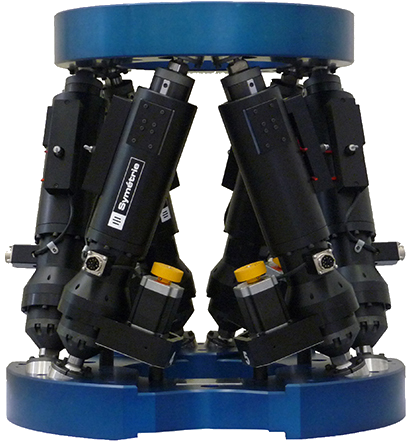
\includegraphics[width=.\linewidth]{fig_01.png}
\end{center}

Ce robot de petite taille évolue directement entre les rangées de cultures pour un travail de précision. Il peut, par exemple, désherber et aussi suivre des personnes lors de la récolte tout en transportant des charges. Bien plus petit qu’un tracteur classique, il ne casse pas la structure naturelle du sol et évite ainsi le phénomène de compaction des sols provoqué habituellement par les tracteurs ou le piétinement de l’homme. Il roule lentement et passe au plus près des cultures sans risquer de les abîmer. Le robot est constitué d’une plate-forme mobile électrique à 4 roues motrices sur laquelle sont fixés divers outils et capteurs. Le moteur du groupe propulsion gauche actionne les 2 roues gauches ensemble et le moteur du groupe propulsion droit actionne les 2 roues droites ensemble, de façon à reproduire finalement un comportement de type « chenilles ». On s’intéresse à l’asservissement de position du robot suivant la ligne moyenne à suivre dans l’allée. On donne les différents modèles de connaissance associés à cet asservissement. 

\begin{center}
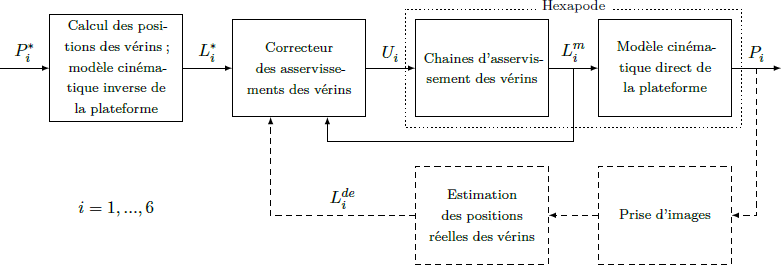
\includegraphics[width=.\linewidth]{fig_02a.png}
\end{center}

\begin{center}
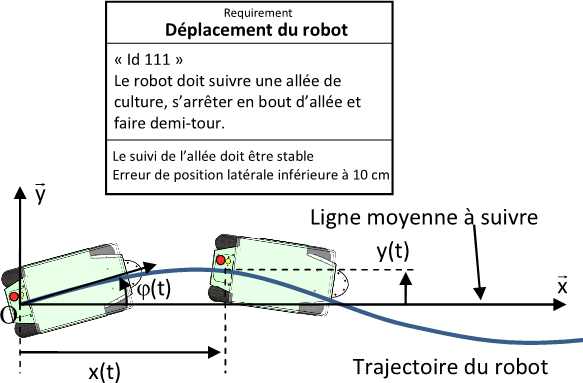
\includegraphics[width=.\linewidth]{fig_02b.png}
\end{center}

La variable $y(t)$ correspond à la distance d’un point particulier du robot par rapport à la ligne moyenne dans le rang de culture. Le modèle de l’asservissement de suivi de l’allée du robot est donné par le schéma-bloc suivant. 

\begin{center}
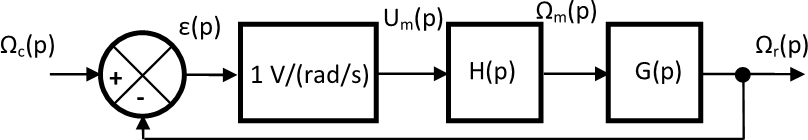
\includegraphics[width=.\linewidth]{fig_03.png}
\end{center}
\fi


\subsection*{Détermination de la fonction de transfert H 1 (p) du groupe propulsion}

On donne dans un premier temps le modèle de connaissance du groupe propulsion gauche. On supposera que toutes les conditions initiales sont nulles et que  $J$,  $R_m$ , $r$, $K_i$, $K_e$ sont des coefficients constants.

\begin{center}
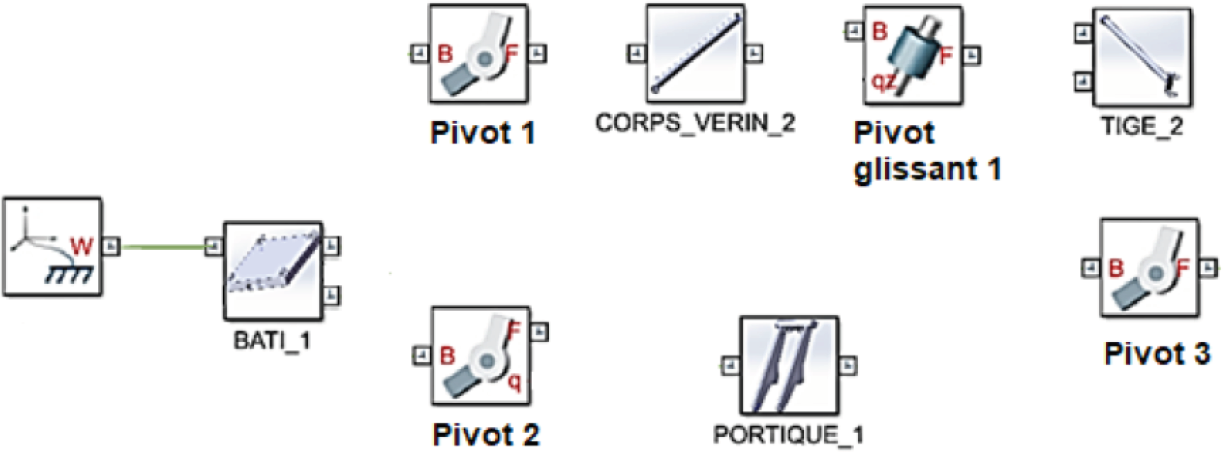
\includegraphics[width=\linewidth]{fig_04.png}
\end{center}

\subparagraph{}
\textit{Appliquer la transformée de Laplace sur les différentes équations du modèle de connaissance.}
\ifprof
\begin{corrige}
\end{corrige}
\else
\fi


\subparagraph{}
\textit{Déduire des questions précédentes le schéma-bloc correspondant au groupe propulsion gauche seul. }
\ifprof
\begin{corrige}
\end{corrige}
\else
\fi

\subparagraph{}
\textit{Déterminer l’expression de la fonction de transfert du système en boucle fermée du groupe propulsion gauche 
$H_g (p) =\dfrac{\Omega_g(p)}{U_g(p)}$ en fonction de $r$, $K_i$, $K_e$, $J$ et $R_m$. Montrer que cette fonction de
transfert peut se mettre sous la forme d’un système du premier ordre $H_g(p)=\dfrac{K}{1+\tau p}$  où $K$ et $\tau$ sont 2
constantes à déterminer. Donner les unités de $K$ et $\tau$. 
} 

\ifprof
\begin{corrige}
\end{corrige}
\else
\fi
Pour faire pivoter le robot d’un angle $\varphi(t)$ autour de l’axe vertical ascendant, il est nécessaire de faire tourner les roues droites et gauches avec 2 vitesses angulaires différentes de façon à reproduire finalement un comportement de type « chenilles ». 

\textbf{Notations}
\begin{itemize}
\item Vitesse angulaire moyenne de rotation des roues : $\omega_r (t)$. 
\item Différence de vitesse de rotation angulaire entre roues droites et roues gauches : $\Delta\omega(t) = \omega_d (t) – \omega_g (t)$.
\item Vitesse de rotation des roues gauches et droites : $\omega_g (t)$ et $\omega_d (t)$ avec $\omega_g (t)  = \omega_r (t)  - \Delta \omega(t)/2$  et $\omega_d (t)  = \omega_r (t)  + \Delta\omega(t)/2$. 
\item La différence de vitesse de rotation entre roues droites et roues gauches, représentée par $\Delta \omega(t)$, permet de contrôler l’orientation du robot, alors que la vitesse moyenne de rotation des roues $\omega_r (t)$  permet de contrôler la vitesse $V(t)$ de déplacement en translation du robot. 
\item Tension de consigne utile pour la rotation : $\Delta U(t)  = U_d (t)  – U_g (t)$. 
\item Tension de consigne des moteurs gauches et droits :
$U_g(t)=U_m (t)-\Delta U(t)/2$
et $U_d (t)=U_m (t)+\Delta U(t)/2$. 
\item Transformées de Laplace des tensions : $U_g (p)$, $U_d (p)$ et $\Delta U(p)$. 
\item Transformées de Laplace des vitesses de rotation : $\Omega_g (p)$, $\Omega_d (p)$ et $\Delta \Omega(p)$. 
\end{itemize}


\subparagraph{}
\textit{A l’aide des relations ci-dessus, déterminer la fonction de transfert en boucle fermée du groupe propulsion 
$H_1(p)=\dfrac{\Delta\Omega(p)}{\Delta U(p)}$. 
Montrer que cette fonction de transfert peut se mettre sous la forme d’un système du premier ordre.}
\ifprof
\begin{corrige}
\end{corrige}
\else
\fi

On donne les tracés de la réponse à un échelon des chaînes de propulsion gauche et droite.  

\begin{center}
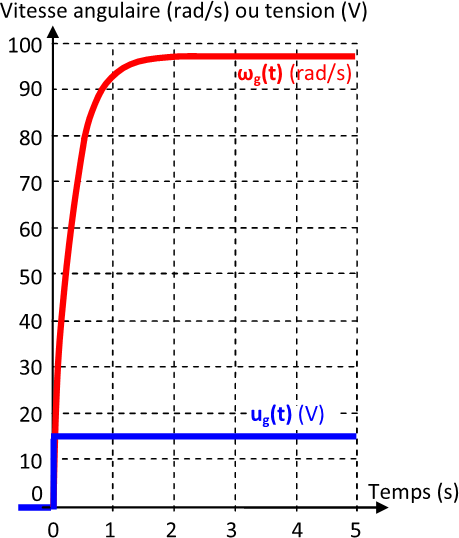
\includegraphics[width=\linewidth]{fig_05a.png}
\end{center}

\begin{center}
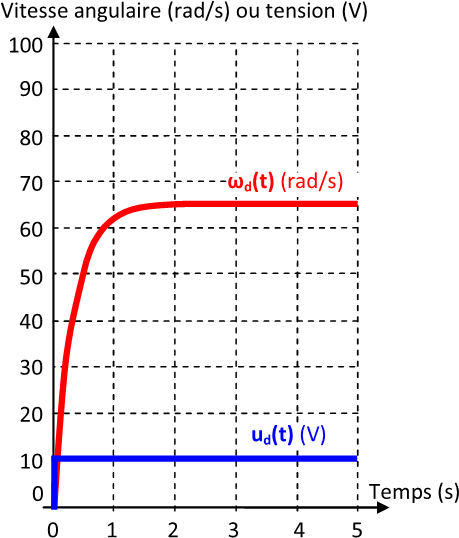
\includegraphics[width=\linewidth]{fig_05b.png}
\end{center}


\subparagraph{}
\textit{Déterminer par identification les expressions des fonctions de transfert $H_g(p) = \dfrac{\Omega_g(p)}{U_g(p)}$ et
$H_d(p) = \dfrac{\Omega_d(p)}{U_d(p)}$.  Donner les valeurs numériques des coefficients de ces fonctions de transfert. }
\ifprof
\begin{corrige}
\end{corrige}
\else
\fi


\subsection*{Détermination de la fonction de transfert $H_2 (p)$ du suivi de la trajectoire}

La modélisation par schéma bloc du suivi de la trajectoire est ci-dessous. La position du robot est repérée dans le plan $\left(O,\vect{x},\vect{y}\right)$ par ses coordonnées $x(t)$ et $y(t)$ ainsi que par l’angle du robot avec la ligne moyenne $\varphi(t)$. 

\begin{center}
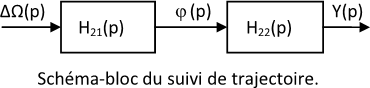
\includegraphics[width=.7\linewidth]{fig_11.png}
\end{center}


On donne le modèle de connaissance du suivi de trajectoire obtenu à l’aide de modèles cinématiques. On supposera que toutes les conditions initiales sont nulles et que e et R sont des coefficients constants. 

\begin{center}
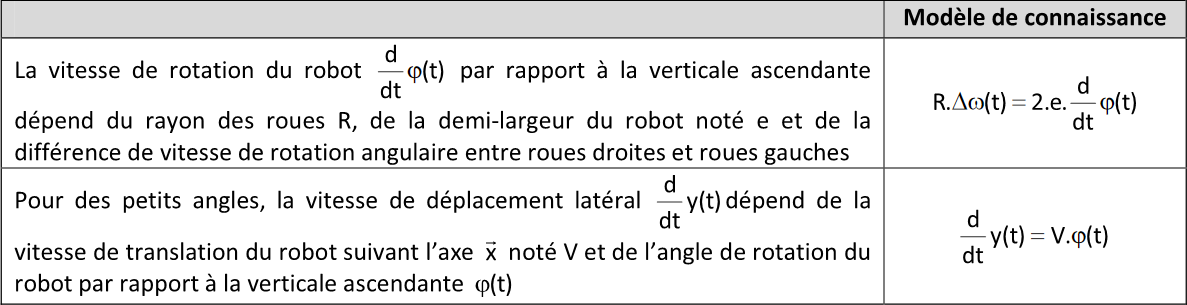
\includegraphics[width=\linewidth]{fig_06.png}
\end{center}


\subparagraph{}
\textit{Appliquer la transformée de Laplace sur les 2 relations cinématiques proposées. }
\ifprof
\begin{corrige}
\end{corrige}
\else
\fi


\subparagraph{}
\textit{ En déduire l’expression des  fonctions de transfert $H_{21} (p)$, $H_{22} (p)$ puis $H_2 (p)$.  }
\ifprof
\begin{corrige}
\end{corrige}
\else
\fi

 \subsection*{Détermination de la fonction de transfert $H_3 (p)$ correspondant au « capteur de distance » }

Les 5 capteurs utilisés pour le guidage dans le  rang de culture sont installés sur un demi-cercle à l’avant du robot : 
\begin{itemize}
\item capteur avant pour la détection des obstacles;
\item capteurs latéraux pour la mesure de distance avec les cultures;
\item capteurs à 45\degres pour la mesure de distance avec avant  anticipation. 
\end{itemize}

\begin{center}
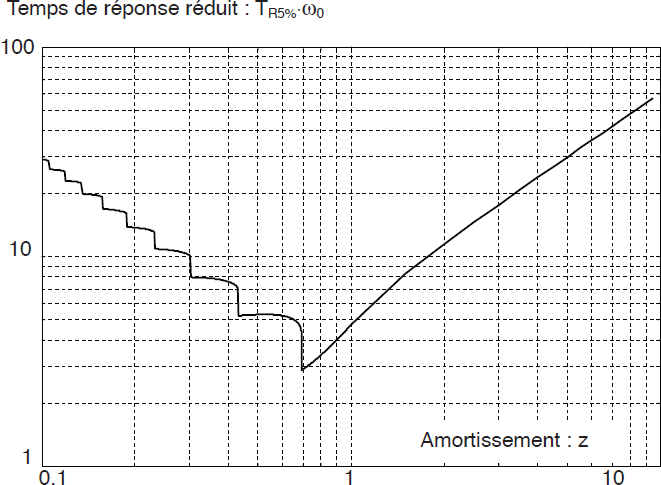
\includegraphics[width=\linewidth]{fig_07.png}
\end{center}

Ces 5 capteurs de distance qui détectent la présence d’objets entre 10 et \SI{80}{cm} sont des capteurs infrarouges type « télémètre ». Ils ont une courbe de réponse $u_{\text{cap}} (t)$ en fonction de la  distance $L$ de l’objet. 

On suppose que seuls les 2 capteurs latéraux sont utilisés pendant le déplacement en ligne droite. Ils sont utilisés en différentiel tel que :  $u_{\text{mes}}(t) = u_{\text{capt gauche}}(t) - u_{\text{capt droit}}(t)$.  

\textbf{Notation} : transformée de Laplace de la tension $u_{\text{mes}} (t)$ : $U_{\text{mes}} (p)$. 

La fonction de transfert $H_3(p) = \dfrac{U_{\text{mes}}(p)}{Y(p)}$ du bloc « capteur de distance » est supposée réduite à un gain pur noté $K_c$ . On note $u_{\text{capt 0}}$ la tension fournie par les 2 capteurs latéraux lorsque le robot est centré entre les 2 rangs de culture distants de \SI{70}{cm}. 

\begin{center}
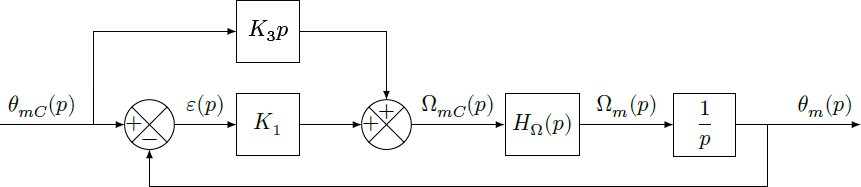
\includegraphics[width=\linewidth]{fig_08.png}
\end{center}

\subparagraph{}
\textit{Réaliser un schéma en vue de dessus permettant de visualiser le robot positionné dans l’allée avec ses 2 capteurs latéraux. Indiquer sur ce schéma les distances entre les capteurs et les rangées de culture.}
\ifprof
\begin{corrige}
\end{corrige}
\else
\fi


\subparagraph{}
\textit{Quelle est la valeur de la tension $u$ à \SI{0,1}{V} près ? Quelle est la tension $u_{\text{capt droit}}$ lorsque le robot est décalé de $y = +\SI{5}{cm}$ suivant l’axe $\vect{y}$ entre ces 2 rangs de culture ? Quelle est la tension $u_{\text{capt gauche}}$ à ce même instant ? }
\ifprof
\begin{corrige}
\end{corrige}
\else
\fi


\subparagraph{}
\textit{En déduire le gain $K_c$ du bloc « capteur de distance » autour de ce point de fonctionnement et préciser son unité.}
\ifprof
\begin{corrige}
\end{corrige}
\else
\fi


\subsection*{Réglage du gain d’adaptation}

Le bloc d’adaptation est un gain proportionnel noté $K_a$ qui permet de convertir la consigne $y_{\text{consigne}}(t)$ en une tension $u_{\text{consigne}}(t)$ image de la consigne.  



\subparagraph{}
\textit{Comment choisir le gain d’adaptation $K_a$ pour que la position $y(t)$ en sortie de l’asservissement soit correctement asservie sur la position de consigne $y_{\text{consigne}} (t)$ (on cherche dans ce cas à obtenir un écart $\varepsilon(p)$ nul lorsque la consigne et la sortie sont égales).}
\ifprof
\begin{corrige}
\end{corrige}
\else
\fi

On considère dans un premier temps que le correcteur est un correcteur proportionnel. On note donc la la fonction de transfert de ce dernier $C(p) = K_p$.


\subparagraph{}
\textit{Déterminer la fonction de transfert boucle ouverte $\text{FTBO}(p)=\dfrac{U_{\text{mes}} (p)}{\varepsilon(p)}$.
Donner la classe et l’ordre de cette fonction de transfert. }
\ifprof
\begin{corrige}
\end{corrige}
\else
\fi

\subsection*{Analyse des performances obtenues.}

On donne ci-dessous la courbe donnant l’évolution du paramètre $y(t)$ sur une allée de \SI{100}{m} pour un premier réglage de correcteur. On donne d’autre part la réponse du véhicule en vitesse de translation pour une consigne échelon de \SI{0,2}{m/s}. 

\begin{center}
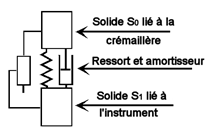
\includegraphics[width=\linewidth]{fig_09.png}
\end{center}


\begin{center}
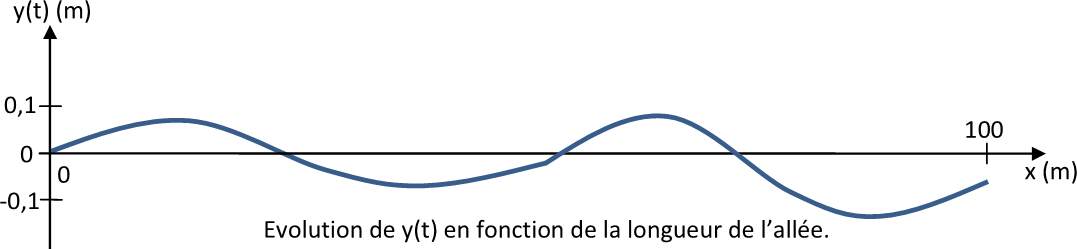
\includegraphics[width=\linewidth]{fig_10.png}
\end{center}

\subparagraph{}
\textit{Déterminer si ce réglage semble adapté vis-à-vis des exigences du cahier des charges. Justifier la réponse en laissant notamment apparaître les tracés utiles sur les courbes. }
\ifprof
\begin{corrige}
\end{corrige}
\else
\fi

\end{multicols}

\begin{center}
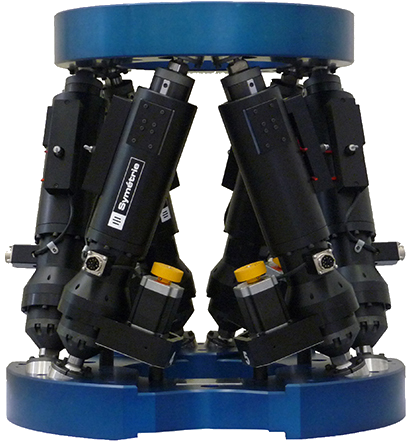
\includegraphics[width=\linewidth]{fig_01.png}
\end{center}
